\documentclass[12pt]{article}
\usepackage{amsmath}
\usepackage{amsfonts}
\usepackage{float}
\usepackage{fancyhdr}
\usepackage{graphicx}
\usepackage[colorlinks=true,linkcolor=blue, citecolor=red]{hyperref}
\usepackage{url}
\usepackage[top=.75in, left=.75in, right=.75in, bottom=1in]{geometry}
\usepackage{multirow}
\usepackage{enumitem}
\usepackage{setspace}
% \usepackage{parskip}
\usepackage{tikz}
\usepackage{forest}

% For algorithm
\usepackage{algorithm}
\usepackage{algpseudocode}

% For table
\usepackage{array}
\usepackage{diagbox}
% ============ CODE ============
\usepackage{listings}
\usepackage{xcolor}
\definecolor{codegreen}{rgb}{0,0.6,0}
\definecolor{codegray}{rgb}{0.5,0.5,0.5}
\definecolor{codepurple}{rgb}{0.58,0,0.82}
\definecolor{backcolour}{rgb}{0.95,0.95,0.92}

\usepackage[backend=biber, sorting=none]{biblatex}
\addbibresource{ref.bib}
\usepackage[inkscapelatex=false]{svg}

% Styling for the code.
\lstdefinestyle{mystyle}{
    backgroundcolor=\color{backcolour},   
    commentstyle=\color{codegreen},
    keywordstyle=\color{magenta},
    numberstyle=\tiny\color{codegray},
    stringstyle=\color{codepurple},
    basicstyle=\ttfamily\footnotesize,
    breakatwhitespace=false,         
    breaklines=true,                 
    captionpos=b,                    
    keepspaces=true,                 
    numbers=left,                    
    numbersep=5pt,                  
    showspaces=false,                
    showstringspaces=false,
    showtabs=false,                  
    tabsize=2
}
\lstset{style=mystyle}

\lstdefinestyle{terminal}{
    basicstyle=\ttfamily\color{black},
    backgroundcolor=\color{gray!10},
    frame=none, % Add top and bottom frames
    framerule=1pt, % Set the frame rule thickness
    framexleftmargin=10pt, % Adjust the left margin of the frame
    breaklines=true,
    breakatwhitespace=true,
    numbers=none, % Remove line numbers
    keepspaces=false, % Keep spaces
    tabsize=2,
}

% Disable indentation on new paragraphs
\setlength{\parindent}{0pt}

% Define course name, report name and report title.
\newcommand{\coursename}{Statistical Machine Learning}
\newcommand{\coursetitle}{STATISTICAL MACHINE LEARNING}
\newcommand{\reportname}{Final Project}
\newcommand{\reporttitle}{FINAL PROJECT}

% Sort by student number
\newcommand{\studentname}{Vu Minh Phat (21127739)\\Trieu Gia Huy (22127166) \\Vo Thanh Nghia (22127295)\\Vo Thinh Vuong (22127464)}
\newcommand{\teachername}{Dr. Ngo Minh Nhut\\TA: Le Long Quoc}

% ============ HEADER AND FOOTER ============
% Header length
\setlength{\headheight}{29.43912pt}

% Footer page number would be on the lower-right corner
\pagestyle{fancy}
\fancyfoot{}
\fancyfoot[R]{\thepage}

\lhead{\reportname}
\rhead{\coursename}

% Set line and paragraph spacing
\renewcommand{\baselinestretch}{1.05}
\setlength{\parskip}{2pt}
\setlength{\parindent}{1.5em} 

% ============ DOCUMENT ============
\begin{document}
\begin{titlepage}
\newcommand{\HRule}{\rule{\linewidth}{0.5mm}}
\centering

\textsc{\LARGE vietnam national university ho chi minh city}\\[0.2cm]
\textsc{\LARGE university of science}\\[0.3cm]
\textsc{\Large faculty of information technology}\\[0.5cm]


\includegraphics[scale=.35]{content/hcmus-logo.png}\\[0.5cm]

% \huge{\bfseries{BÁO CÁO}}\\
\huge{\bfseries{DATA REPRESENTATION}}\\
\textbf{\large COURSE NAME: \coursetitle}\\[0.5cm]

\begin{minipage}[t]{0.45\textwidth}
\begin{flushleft} \large
\emph{Student:}\\
\studentname
\end{flushleft}
\end{minipage}
~
\begin{minipage}[t]{0.45\textwidth}
\begin{flushright} \large
\emph{Lecturer:} \\
\teachername
\end{flushright}
\end{minipage}\\[5cm]

{\large \today}\\[2cm]


\vfill
\end{titlepage}
	

\setcounter{tocdepth}{3}

\tableofcontents
\pagebreak

\section{Information}
\subsection{Student Information}
\renewcommand{\arraystretch}{2}

\begin{center}
\begin{tabular}{|>{\centering\arraybackslash}m{4cm}|>{\centering\arraybackslash}m{5cm}|>{\centering\arraybackslash}m{7cm}|}
  \hline
  \textbf{\Large Student ID} & \textbf{\Large Full name} & \textbf{\Large Email} \\
  \hline
  \Large 22127166 & \Large Trieu Gia Huy & \Large tghuy22@clc.fitus.edu.vn
  \\
  \hline
  \Large 22127295 & \Large Vo Thanh Nghia & \Large vtnghia22@clc.fitus.edu.vn \\
  \hline
  \Large 22127464 & \Large Vo Thinh Vuong & \Large vtvuong22@clc.fitus.edu.vn \\
  \hline  
  \Large 21127739 & \Large Vu Minh Phat & \Large vmphat21@clc.fitus.edu.vn \\
  \hline    
\end{tabular}
\end{center}

\subsection{Source Code}

\href{https://github.com/nghessss/CSC15004-StatisticalML}{GitHub}

\section{Introduction}

\subsection{Background and Motivation}

In the current digital age, we are witnessing an explosion of multimedia data, especially videos. From social media platforms like YouTube, TikTok, and Facebook to security surveillance systems, online courses, and personal archives, video has become a popular and effective medium for conveying information. However, the vast amount of information contained within these videos presents a major challenge: how can we access and retrieve specific information quickly and accurately?

Traditional search methods typically rely on human-created \textbf{metadata}, such as titles, descriptions, or tags. This approach is limited when users want to find specific details inside a video's content, such as a particular action, an object that appears for only a few seconds, the color of an item, or a sentence spoken at a specific moment. Watching an entire video just to find one piece of information is extremely time-consuming and inefficient.

To solve this problem, Artificial Intelligence (AI) technologies, particularly in the fields of \textbf{Computer Vision (CV)} and \textbf{Natural Language Processing (NLP)}, have introduced groundbreaking solutions. Models that can ``understand'' the content of images and videos (Image/Video Captioning) and ``listen'' to audio (Speech Recognition) are becoming increasingly powerful and precise.

Driven by this practical need, this project proposes the development of an \textbf{intelligent chatbot system that allows users to directly ask questions about the content of a video}. Instead of watching the entire video, users can interact with the system using natural language, asking questions and receiving accurate answers based on both the visual and audio content of the video.

\subsection{Project Objectives}

This project aims to solve the problem of detailed information retrieval from videos by building and integrating an intelligent chatbot system. The specific objectives are as follows:

\paragraph{Build a Comprehensive Context for Videos:} To automatically extract and combine information from three primary sources:

\begin{itemize}
    \item \textbf{Static Visual Content (Image Captioning):} Summarize the general scene, main objects, and their attributes from key frames of the video.
    
    \item \textbf{Action-based Content (Video Captioning):} Describe the actions and events happening in the video using a specialized model (\textbf{BTKG}~\cite{btkg}) designed to capture motion.
    
    \item \textbf{Audio Content (Speech Recognition):} Convert all speech and dialogue within the video into a text transcript using \textbf{PhoWhisper}, a high-accuracy Vietnamese speech recognition model.
\end{itemize}

\paragraph{Develop an Interactive Chatbot:} To build a chatbot that can understand user questions in natural language and use the generated context to find and provide appropriate answers.

\paragraph{Integrate and Test the System:} To combine the individual modules (Image Captioning, Video Captioning, PhoWhisper, and Chatbot) into a single, complete system and test its effectiveness through real-world question-and-answer scenarios.

\subsection{Proposed Architecture and Solution}

To achieve the objectives mentioned above, the proposed system consists of several core components that work together to create a complete information processing workflow.

\subsubsection*{System Workflow:}

When a user uploads a video, the system processes it using three core modules in parallel:

\begin{enumerate}
    \item \textbf{Image Captioning Module:} The system extracts several key frames that represent the overall scenery of the video. These frames are then fed into an Image Captioning model to generate short descriptive sentences. For example, from a video of someone at a gym, this module might generate the description: ``\textit{A man is in a gym with various equipment}''. The purpose of this module is to summarize the static scene and objects.
    
    \item \textbf{Video Captioning Module (based on the BTKG model):} The entire video is analyzed by the Video Captioning model. This model is specifically designed to focus on recognizing motion and actions. The output is one or more sentences describing the main events. For example: ``\textit{A man is lifting weights}''. This module answers the question, ``What is happening?''.
    
    \item \textbf{Speech Recognition Module (PhoWhisper):} The audio stream from the video is separated and processed by the PhoWhisper model. This model converts all conversations or spoken words in the video into a full text transcript. For instance, if the person in the video says, ``\textit{Today, I will try the 100kg weights}'', this module will produce that exact text.
\end{enumerate}

These three outputs (the static scene description, the action description, and the audio transcript) are then combined to create a single, comprehensive \textbf{text context}. This context acts as the ``brain'' of the chatbot.

When a user asks a question, the chatbot analyzes the query and searches within this text context to provide the most accurate answer.

\subsubsection*{Illustrative Example:}

Consider a video of a person lifting weights. The system would generate a context similar to this:

\begin{itemize}
    \item \textbf{Image Captioning:} ``A man wearing a blue shirt and black pants is in a gym.''

    \item \textbf{Video Captioning:} ``The man is performing an overhead weightlifting press.''

    \item \textbf{PhoWhisper Transcript:} ``(Sound of breathing) Come on... just one more rep.''
\end{itemize}

\noindent
Based on this context, the chatbot can answer a variety of user questions:

\begin{itemize}
    \item \textbf{User asks:} ``What color is the person's shirt?''
    \begin{itemize}
        \item \textbf{Chatbot answers:} ``The person in the video is wearing a blue shirt.'' (Data from Image Captioning)
    \end{itemize}

    \item \textbf{User asks:} ``What is that person doing?''
    \begin{itemize}
        \item \textbf{Chatbot answers:} ``The person in the video is performing an overhead weightlifting press.'' (Data from Video Captioning)
    \end{itemize}

    \item \textbf{User asks:} ``Is this person saying anything?''
    \begin{itemize}
        \item \textbf{Chatbot answers:} ``Yes, the person says: `Come on... just one more rep'.'' (Data from PhoWhisper)
    \end{itemize}
\end{itemize}

% Kiến trúc của mô hình 
\section{Bidirectional Transformer with Knowledge Graph (BTKG)}
\label{sec:archi}

\subsection{Overview}

This section describes the proposed Bidirectional Transformer with Knowledge Graph (BTKG) model~\cite{btkg} (Figure~\ref{fig:archi}). We begin by reviewing the basic transformer module and how video features are extracted and captions generated. We then detail the BTKG architecture, including the Spatio-Temporal Encoder, the Objects and Relationships Encoder, and the bidirectional decoder (Backward and Forward Decoders). Finally, we explain the training strategy, including pseudo reverse captions and the loss functions.

\begin{figure}[H]
    \centering
    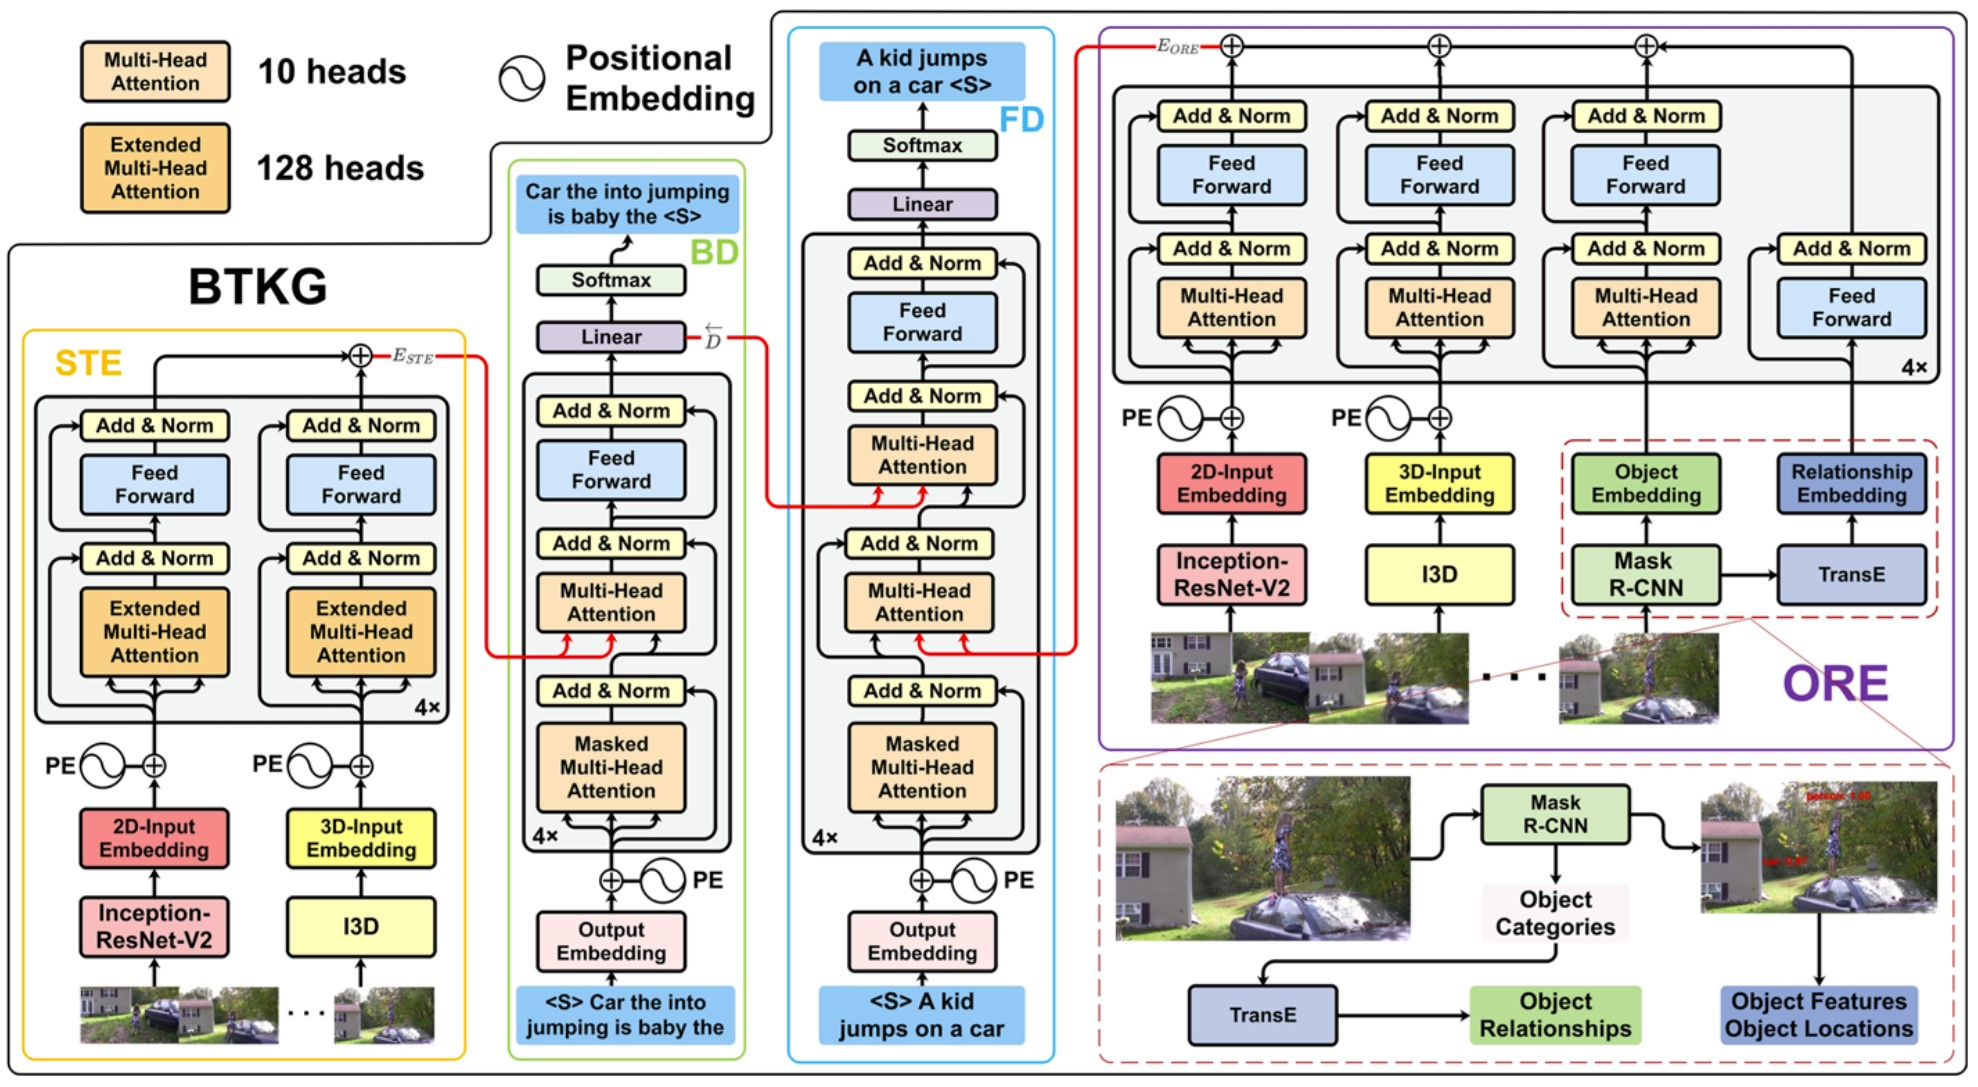
\includegraphics[width=1\linewidth]{image/archi.jpg}
    \caption{The figure illustrates the proposed BTKG based on the transformer architecture in detail, which consists of Spatio-Temporal Encoder (STE), Objects and Relationships Encoder (ORE), Backward Decoder (BD), and Forward Decoder (FD).}
    \label{fig:archi}
\end{figure}

\subsection{Basic Module}

\subsubsection{Transformer Architecture}

The model is built upon the standard Transformer~\cite{attention_is_all_you_need} architecture. A Transformer consists of an encoder and a decoder, each formed by stacking identical layers. Within each layer are two sub-layers: a multi-head attention (MHA) mechanism and a position-wise feed-forward network (FFN), each followed by residual connections and layer normalization. In the MHA sub-layer, the input queries ($Q$), keys ($K$), and values ($V$) are linearly projected into multiple ``heads''. Specifically, for head $i$, we compute $Q W_i^Q$, $K W_i^K$, and $V W_i^V$, where $W_i^Q,W_i^K,W_i^V$ are learned projection matrices. The attention outputs of the $h$ heads are concatenated and projected via $W^O$:
\begin{equation}
\begin{split}
\mathrm{MultiHead}(Q,K,V)
  &= \mathrm{Concat}(\mathrm{head}_1,\dots,\mathrm{head}_h)\,W^O,\\
\mathrm{head}_i
  &= \mathrm{Attention}(QW_i^Q,\,KW_i^K,\,VW_i^V).
\end{split}
\label{eq:mha}
\end{equation}

The Attention function uses scaled dot-product attention:
$$
\mathrm{Attention}(Q_i,K_i,V_i) \;=\; \mathrm{softmax}\Big(\frac{Q_iK_i^T}{\sqrt{d_k}}\Big)\,V_i,
$$
where $d_k$ is the dimensionality of the key vectors.

The FFN sub-layer applies two linear transformations with a ReLU nonlinearity in between. For an input $X$,
$$
\mathrm{FFN}(X) = \max(0,\,XW_1 + b_1)\,W_2 + b_2,
$$
with parameters $W_1,W_2,b_1,b_2$. Together, these MHA and FFN components provide the basic sequence modeling capability of the Transformer.

\subsubsection{Multimodal Features Extraction and Captions Generation}

The task is video captioning, so the model must encode both visual and dynamic information. To this end, the system extracts \textbf{image features} and \textbf{motion features} from the video. It uses the Inception-ResNet-V2 network (pretrained on ImageNet) to extract per-frame image features, capturing static appearance. For motion, it uses the Inflated 3D ConvNet (I3D) pretrained on the Kinetics dataset to extract features from sequences of frames (capturing temporal dynamics). These networks produce feature sequences $F_I=\{f_1,\dots,f_L\}$ and $F_M=\{v_1,\dots,v_N\}$, where $f_i\in\mathbb{R}^{d_I}$ are image features for $L$ sampled frames and $v_j\in\mathbb{R}^{d_M}$ are motion features (with $N=L/64$ in practice). Both feature sequences are then projected into a common model dimension $d_{model}$ via learned linear mappings.

In addition to these frame-level features, the model incorporates \textbf{object-level semantics}. A Mask R-CNN detector (trained on the COCO dataset) detects objects in each frame and produces object feature vectors and class labels. For each detected object, its class name (e.g. ``car'', ``person'') is used in a knowledge graph module: a TransE-based model predicts relationships (triplets) between object categories. The object labels and their predicted relations are embedded via a shared word-embedding matrix (e.g. Word2Vec) to produce relation features.

For caption generation, this base module uses a bidirectional decoding strategy~\cite{BiTransformer}: there is a backward decoder and a forward decoder. The backward decoder generates captions right-to-left (reverse order), while the forward decoder generates left-to-right. This bidirectional decoder takes as input the encoded video features. The backward decoder's output (a reverse caption and its hidden context) is fed into the forward decoder to improve forward captioning. In summary, the basic module provides: a Transformer backbone, multimodal feature encodings (image, motion, objects, relations), and a bidirectional decoding scheme.

\subsection{BTKG Architecture}

The BTKG model integrates the above components into a unified architecture. It connects a bidirectional decoder with an encoder that incorporates knowledge-graph-enriched object features. As shown in Figure~\ref{fig:archi}, BTKG consists of four parts:

\begin{itemize}[nosep]
    \item \textbf{Spatio-Temporal Encoder (STE):} encodes fine-grained frame and motion features to produce $E_{STE}$.
    
    \item \textbf{Objects and Relationships Encoder (ORE):} encodes object features and their relationships (along with coarse video features) to produce $E_{ORE}$.
    
    \item \textbf{Backward Decoder (BD):} generates a reverse caption $Y_{BD}$ (right-to-left) and outputs a hidden context $\overleftarrow{D}$.
    
    \item \textbf{Forward Decoder (FD):} generates the final caption $Y_{FD}$ (left-to-right), integrating both $E_{ORE}$ and the reverse context $\overleftarrow{D}$.
\end{itemize}

The next subsections explain each component in detail.

\subsubsection{Spatio-Temporal Encoder (STE)}

The STE is designed to capture the fine-grained spatio-temporal content of the video. It operates on the image and motion feature sequences extracted from the video frames (as described above). Formally, let $X=\{x_1,\dots,x_L\}$ be the sampled frames. We extract image features
$$
F_I = \{f_1,\dots,f_L\}, \quad f_i\in\mathbb{R}^{d_I},
$$
and motion features
$$
F_M = \{v_1,\dots,v_N\}, \quad v_j\in\mathbb{R}^{d_M}, \quad N = L/64,
$$
using Inception-ResNet-V2 and I3D respectively. To combine these modalities, each feature vector is linearly projected to a common dimension $d_{\text{model}}$ by learned weights:
$$
f'_i = W_L f_i + b_L,\quad v'_j = W_N v_j + b_N,
$$
where $W_L\in\mathbb{R}^{d_{\text{model}}\times d_I}$, $W_N\in\mathbb{R}^{d_{\text{model}}\times d_M}$, and biases $b_L,b_N\in\mathbb{R}^{d_{\text{model}}}$. This yields transformed sequences $F'_I = \{f'_1,\dots,f'_L\}$ and $F'_M = \{v'_1,\dots,v'_N\}$, where $f'_i, v'_j \in \mathbb{R}^{d_{\text{model}}}$.

The sequences $F'_I$ and $F'_M$ are then each fed through a Transformer encoder (with self-attention and FFN sublayers) to produce embeddings $E_I \in\mathbb{R}^{L\times d_{\text{model}}}$ and $E_M \in\mathbb{R}^{N\times d_{\text{model}}}$. Finally, these are fused by element-wise addition to produce the STE output:
$$
E_{STE} = E_I \oplus E_M,
$$
where $\oplus$ denotes element-wise sum. Thus $E_{STE}\in\mathbb{R}^{L\times d_{\text{model}}}$ encodes frame-level (fine-grained) video content by blending appearance and motion features.

A notable detail is that in the STE, the model uses an \textbf{extended multi-head attention} with 128 heads (instead of the usual 8). Using more heads allows the model to capture correlations among positions at a finer temporal scale than whole frames. In practice, the STE employs $h=128$ attention heads as indicated in Eq.~\ref{eq:mha}, which helps BTKG capture fine temporal dependencies.

\subsubsection{Objects and Relationships Encoder (ORE)}

The ORE captures higher-level semantics by encoding detected objects and their relationships. First, objects are detected in the video using Mask R-CNN (with a Feature Pyramid Network and ROI pooling). For each detected object $i$ (up to $k$ objects), we record its normalized bounding box coordinates and a visual feature vector. Let $R_l=[l_1,\dots,l_k]$ be the list of object locations (each $l_i$ is 4-dimensional) and $R_v=[v_1,\dots,v_k]$ the list of object feature vectors. These are concatenated per-object: the $i$-th object feature is $(l_i|v_i)$, and stacking these forms the object feature matrix $F_o$:
$$
F_o = \mathrm{concat}_{i=1}^k\bigl(l_i,\,v_i\bigr).
$$
in the paper's notation this is written as
$$
F_o = \mathrm{concat}_{i=1,\dots,k}(R_l\,R_v),
$$
meaning the row-wise concatenation of $R_l$ and $R_v$ for each object.

In parallel, the object class labels (one-hot vectors $o_i$) are input to the TransE knowledge graph model to predict relations between objects. This yields a set of relation one-hot vectors $\{r_1,\dots,r_{m}\}$, where $m=\binom{k}{2}$. Both the object labels $o_i$ and relation labels $r_j$ are embedded into the same vector space via a shared embedding matrix $W$ (pretrained by Word2Vec). Specifically:
$$
o'_i = o_i W,\quad r'_j = r_j W,
$$
producing embedded matrices $R'_o=[o'_1,\dots,o'_k]$ and $R'_r=[r'_1,\dots,r'_m]$. These are concatenated vertically to form the relation feature matrix $F_r$:
$$
F_r = \begin{bmatrix}R'_o \\ R'_r\end{bmatrix}
$$

The matrix $F_r$ thus contains semantic features of objects and predicted relations.

Next, the ORE encodes the content of $F'_I$, $F'_M$ (the same projected image/motion features as STE), $F_o$, and $F_r$. As in the STE, $F'_I$ and $F'_M$ are passed through transformer encoders (here using 10 attention heads) to yield embeddings $E_I$ and $E_M$. Then the object feature matrix $F_o$ is encoded (via a transformer encoder without positional encoding, since object order is arbitrary) to produce an object embedding $E_o$. Likewise, the relation matrix $F_r$ is encoded by a simple feed-forward network (no attention, since relations are unordered) to produce a relation embedding $E_r$.

Finally, these four embeddings are fused by element-wise addition:
$$
E_{ORE} = E_I \oplus E_M \oplus E_o \oplus E_r.
$$

This sum is the output of the ORE. Thus $E_{ORE}\in\mathbb{R}^{L\times d_{\text{model}}}$ encodes coarse video features (from $E_I,E_M$) enriched by object and relation semantics ($E_o,E_r$).

\subsubsection{Backward Decoder (BD)}

The Backward Decoder generates a caption in reverse order (right-to-left). It takes the STE output $E_{STE}$ as its encoder memory; it does not use $E_{ORE}$, because object relations have no natural reverse-time ordering and could confuse the backward generation. The BD is implemented as a transformer decoder: at each step it attends to $E_{STE}$ and generates one word from the end of sentence toward the beginning. Generation stops when the end marker $<S>$ is produced. If the generated reverse caption is $\overleftarrow{C} = [s_1, s_2, \dots, s_L, <S>]$, then the final hidden state of the BD (after producing $s_L$) is denoted $\overleftarrow{D}_L$. We define the BD's context output as
$$
\overleftarrow{D} = \overleftarrow{D}_L
$$
This vector $\overleftarrow{D}$ summarizes the reverse caption's context and is passed on to the forward decoder.

\subsubsection{Forward Decoder (FD)}

The Forward Decoder generates the final caption left-to-right. It integrates two sources of context: the video encoding and the backward decoder's context. Concretely, the FD attends to $E_{ORE}$ (via a standard encoder-decoder attention) so that object and relation features inform each predicted word. It also attends to the reverse caption context $\overleftarrow{D}$ via an extra cross-attention layer. In practice, at each step the FD takes as input all previously generated words and uses cross-attention over $\overleftarrow{D}$ so that it ``sees'' the whole reverse caption context. It similarly attends to $E_{ORE}$ (which contains object/relation/video info). Generation ends at $<S>$, producing a forward caption $\overrightarrow{C}=[s_1,\dots,s_T,<S>]$. Thus, the FD effectively conditions each word on both $E_{ORE}$ and $\overleftarrow{D}$.

\subsection{Proposed Enhancements}

\subsubsection{Learnable Multimodal Feature Fusion}

\subsubsection*{Background and Limitation}

In the original BTKG architecture, multimodal features are combined using element-wise addition. Specifically, the Spatio-Temporal Encoder (STE) fuses image and motion features via the formula:
$$E_{STE} = E_I \oplus E_M$$

Similarly, the Objects and Relationships Encoder (ORE) combines all four feature types as:
$$E_{ORE} = E_I \oplus E_M \oplus E_o \oplus E_r$$

This method has an inherent limitation: it assumes that each modality contributes equally to the final representation. Element-wise addition is a static, non-learnable operation that cannot dynamically adjust the weight of each feature type based on the video's context.

\subsubsection*{Proposed Solution: Feature Fusion Module}

To overcome this drawback, we replace the element-wise addition with a learnable \textbf{Feature Fusion} module. This module employs a 1D convolutional layer (\texttt{Conv1D}) with a kernel size of 1, which effectively acts as a shared linear layer to intelligently combine features.

The \textbf{Feature Fusion} module operates as follows:
\begin{enumerate}[nosep]
    \item \textbf{Concatenation}: Instead of adding them, the feature tensors from different modalities (e.g., $E_I, E_M, E_o, E_r$), which share the shape \texttt{(batch\_size, seq\_len, d\_model)}, are concatenated along the last dimension. This creates a new tensor of shape \texttt{(batch\_size, seq\_len,\\ n\_features * d\_model)}, where \texttt{n\_features} is the number of modalities.
    
    \item \textbf{1x1 Convolution}: The concatenated tensor is then passed through a \texttt{Conv1D} layer with a kernel size of 1. This convolutional layer serves as a learnable linear projection, mapping the feature space from \texttt{n\_features * d\_model} back down to \texttt{d\_model}. In essence, it learns how to ``mix'' the concatenated features to produce a new, more concise, and meaningful representation.
    
    \item \textbf{Output Reshaping}: The output tensor from the \texttt{Conv1D} layer has the shape \texttt{(batch\_size, seq\_len, d\_model)}, making it fully compatible with the rest of the Transformer architecture and a direct replacement for the previous element-wise sum.
\end{enumerate}

\subsubsection*{Advantages of this Improvement:}
\begin{itemize}[nosep]
    \item \textbf{Learnability}: The weights of the \texttt{Conv1D} layer are updated during training. This allows the model to automatically learn the relative importance of each feature type. For instance, in a video with complex actions, the model might learn to assign higher weights to motion features ($E_M$) and relationship features ($E_r$).
    
    \item \textbf{Enhanced Representation Power}: By allowing features to interact through a learned linear transformation, the model can create a richer and more expressive joint representation space compared to a simple summation.
    
    \item \textbf{Computational Efficiency}: A 1x1 convolution is a highly efficient operation that does not significantly increase the model's computational cost or complexity but substantially improves its expressive power.
\end{itemize}

\subsubsection{Improving the Transformer Architecture with ResiDual Connections}

\subsubsection*{Background and Problem}

The Transformer architecture in the original BTKG model utilizes \textbf{Post-Layer Normalization (Post-LN)}. In this structure, a residual connection is performed by adding the input and output of a sub-block (e.g., Multi-Head Attention), after which Layer Normalization is applied.

While common, the Post-LN architecture suffers from critical limitations, especially when building deep models:

\begin{enumerate}
    \item \textbf{Gradient Vanishing}: As the gradient signal backpropagates from the top layers to the bottom ones, its magnitude decays exponentially. This is because the gradient must pass through numerous Layer Normalization operations, which hinders the effective training of deeper layers.
    
    \item \textbf{Training Instability}: Successfully training deep Post-LN Transformers often requires auxiliary techniques like learning-rate warm-up to mitigate instability in the early stages of training.
\end{enumerate}

\subsubsection*{Proposed Solution: Adopting the ResiDual Architecture}

To address these issues and enhance model stability and performance, we replaced the original Post-LN architecture with \textbf{ResiDual}, an advanced architecture proposed by Xie et al. (2023)~\cite{ResiDual} at Microsoft. ResiDual is designed to combine the advantages of both Post-LN and Pre-Layer Normalization (Pre-LN) while eliminating their respective drawbacks.

\begin{figure}[H]
    \centering
    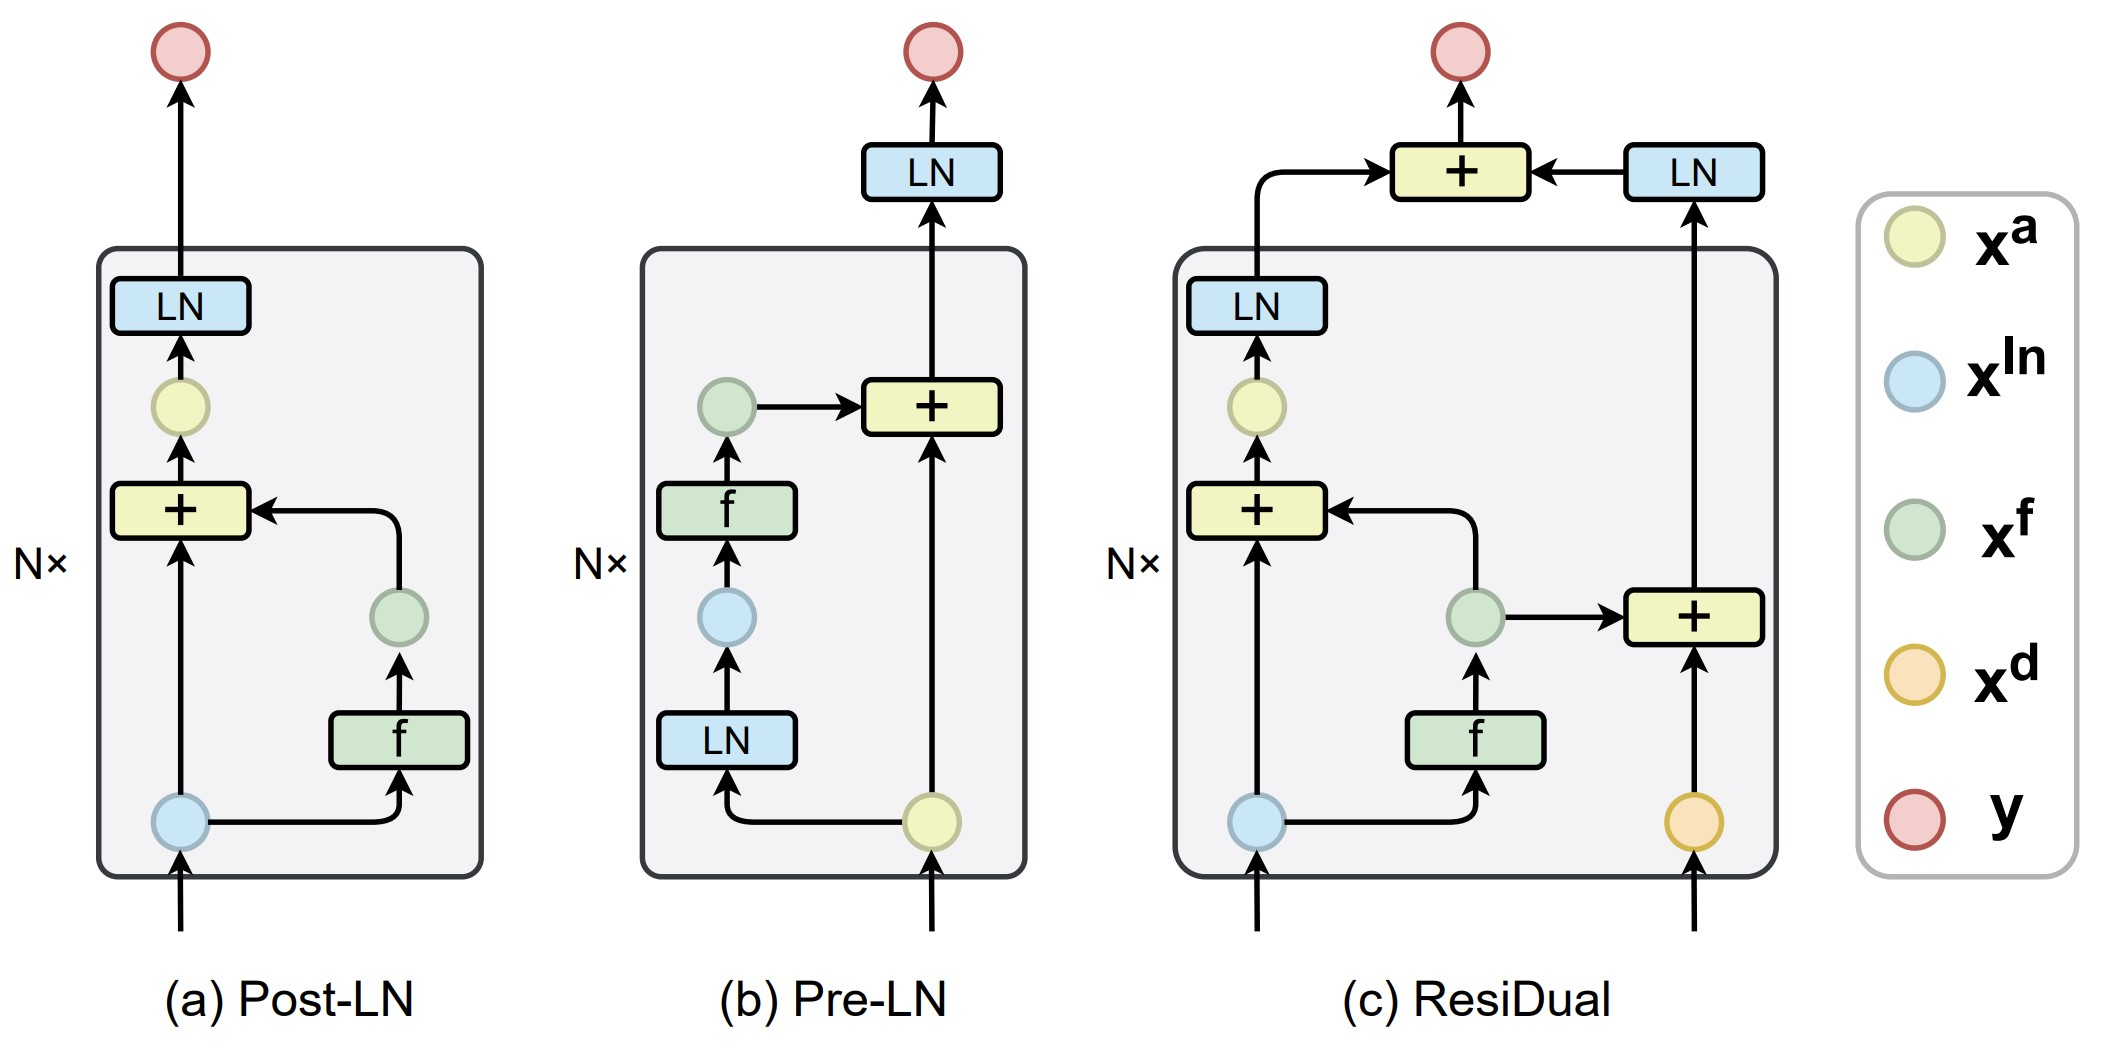
\includegraphics[width=1\linewidth]{image/residual.jpg}
    \caption{Overview of Post-LN, Pre-LN, and ResiDual. Circles with different colors represent different variables and rectangles represent different operations.}
    \label{fig:residual}
\end{figure}

The ResiDual architecture utilizes \textbf{two parallel residual branches}:

\begin{itemize}
    \item \textbf{Main Branch (Post-LN-like)}: This branch retains the structure of Post-LN, where the sub-block's output is added to its input and then normalized. This branch is crucial for \textbf{maintaining representation diversity}, which helps combat the ``representation collapse'' phenomenon often observed in Pre-LN.
    
    \item \textbf{Dual Branch (Pre-LN-like)}: A second residual path is added, allowing the signal (both forward and backward) to bypass the blocks. This branch accumulates the outputs of the sub-blocks and allows the gradient to flow directly to the deepest layers without being attenuated by normalization layers. This effectively \textbf{solves the gradient vanishing problem}.
\end{itemize}

\subsubsection*{Benefits of Adopting ResiDual:}

\begin{itemize}
    \item \textbf{Stable Training and Better Convergence}: By providing an unimpeded path for the gradient, ResiDual makes the training process significantly more stable, especially as model depth increases. This reduces the dependency on techniques like learning-rate warm-up.

    \item \textbf{Enhanced Representation Capacity}: The architecture prevents representation collapse, ensuring that deeper layers can continue to effectively learn and refine features. This allows the model to fully leverage its parameters, leading to a more powerful and robust model.
\end{itemize}

\subsection{Training}

BTKG is trained end-to-end with cross-entropy losses on both decoders. The training involves a two-stage process: first use the backward decoder to generate (pseudo) reverse captions, then use those in the forward decoder. Let $D$ be the training set of videos with forward ground-truth captions. For each video $V$ with forward caption $\overrightarrow{Y}=[y_1,\dots,y_L]$, we first obtain a pseudo reverse caption (described below) and train the BD on that. The FD is then trained on the forward caption, conditioned on the BD's output. Denote the BD loss by $L_{bd}$ and the FD loss by $L_{fd}$ (both standard token-level cross-entropy). The total training loss is a weighted sum:
$$
L = (1-\lambda)\,L_{bd} + \lambda\,L_{fd},
$$
where $\lambda\in[0,1]$ balances the two parts.

\subsubsection{Pseudo Reverse Captions}

To avoid trivial information leakage, the reverse captions used for training are pseudo. All ground-truth forward captions for a video are reversed in order (word sequence flipped) to create candidate reverse captions of the same length. Then these reversed captions are randomly shuffled and paired with the original video, so the final training reverse caption is not exactly the true reverse of its forward caption. In other words, for training we do not feed the exact future ground-truth to the BD. This randomization mitigates the leakage issue and prevents the model from cheating by memorizing exact reversals.

\subsubsection{Backward Decoder Loss}

The BD is trained to minimize the negative log-likelihood of the pseudo reverse captions. Formally, if $(V,\overleftarrow{Y})\in D$ where $\overleftarrow{Y}$ is a training reverse caption (of length $T$), then
$$
L_{bd} = \sum_{(V,\overleftarrow{Y})\in D}\;\sum_{t=1}^T -\log p(y_t \mid V,\,y_1,\dots,y_{t-1};\;\theta_{ste},\theta_{bd}),
$$
where $y_t$ is the $t$-th token in $\overleftarrow{Y}$, and $\theta_{ste},\theta_{bd}$ are the STE and BD parameters. This is the standard cross-entropy loss for the backward decoder.

\subsubsection{Forward Decoder Loss}

Similarly, the FD is trained by cross-entropy on the forward captions. Importantly, each forward token probability is conditioned on both the video and the reverse-context $\overleftarrow{D}$. The loss is:
$$
L_{fd} = \sum_{(V,\overrightarrow{Y})\in D}\;\sum_{l=1}^L -\log p(y_l \mid V,\,y_1,\dots,y_{l-1};\;\theta_{ste},\theta_{bd},\theta_{ore},\theta_{fd}),
$$
with $\theta_{fd},\theta_{ore}$ the FD and ORE parameters. Though the form looks like a normal forward loss, recall that in the FD decoder architecture each step attends to $\overleftarrow{D}$ (the BD context), allowing the model to use ``future'' information encoded by the BD.

In summary, training optimizes $L = (1-\lambda)L_{bd} + \lambda L_{fd}$ so that the BD learns to generate accurate reverse captions and the FD learns to generate accurate forward captions given both video features and the reverse-context. This bidirectional setup with pseudo-reverse captions is designed to reduce information leakage and fully exploit the video semantics captured by the Knowledge Graph encoder.
\section{Keyframe-Based Image Captioning}

% We also explore a different approach to video captioning, focusing on keyframe-based image captioning. This method leverages the strengths of image captioning models to generate captions for selected keyframes from videos, rather than processing the entire video sequence.

Beyond the primary video-level architecture, we further investigate a complementary paradigm that treats video captioning as a sequence of keyframe-driven image-captioning tasks. In this variant, keyframes are first distilled from the clip and each is captioned by a image-captioning model, rather than processing the entire video sequence. 


\subsection{Keyframe Selection}

The keyframe selection procedure is designed to minimize redundancy and extract only those frames that represent significant visual changes within the video. This process involves the following steps:

\begin{enumerate}[nosep]
    \item Frame Sampling: Frames are initially sampled from the video at a rate of 1 frame per second (fps). This sampling rate substantially reduces the processing load while maintaining a linear runtime relative to the video duration, which is well-suited for short, single-activity videos typical of the MSVD dataset.
    \item Feature Extraction via Visual Embedding: Each sampled frame is transformed into a high-dimensional feature vector using a Vision Transformer (google/vit-base-patch16-224-in21k~\cite{google-vit-base-patch16-224-in21k}) model pre-trained on the ImageNet-21k dataset. ViT embeddings were selected for their demonstrated robustness to common visual artifacts such as motion blur and variations in illumination, rendering them a reliable foundation for change detection.
    \item Similarity-Based Filtering: A frame is designated as a keyframe if its visual representation is sufficiently dissimilar from that of the preceding keyframe. This determination is made using a cosine similarity metric. A frame is added to the keyframe set if the cosine similarity score between its embedding and that of the last accepted keyframe is below a threshold of 0.95.
\end{enumerate}



\subsection{Image Captioning Model}

\subsubsection{Model Architecture}
The image captioning model employs a sophisticated encoder-decoder architecture, integrating a pre-trained Vision Transformer (ViT) as the encoder and a pre-trained Transformer-based language model (T5) as the decoder.

\begin{figure}
  \centering
  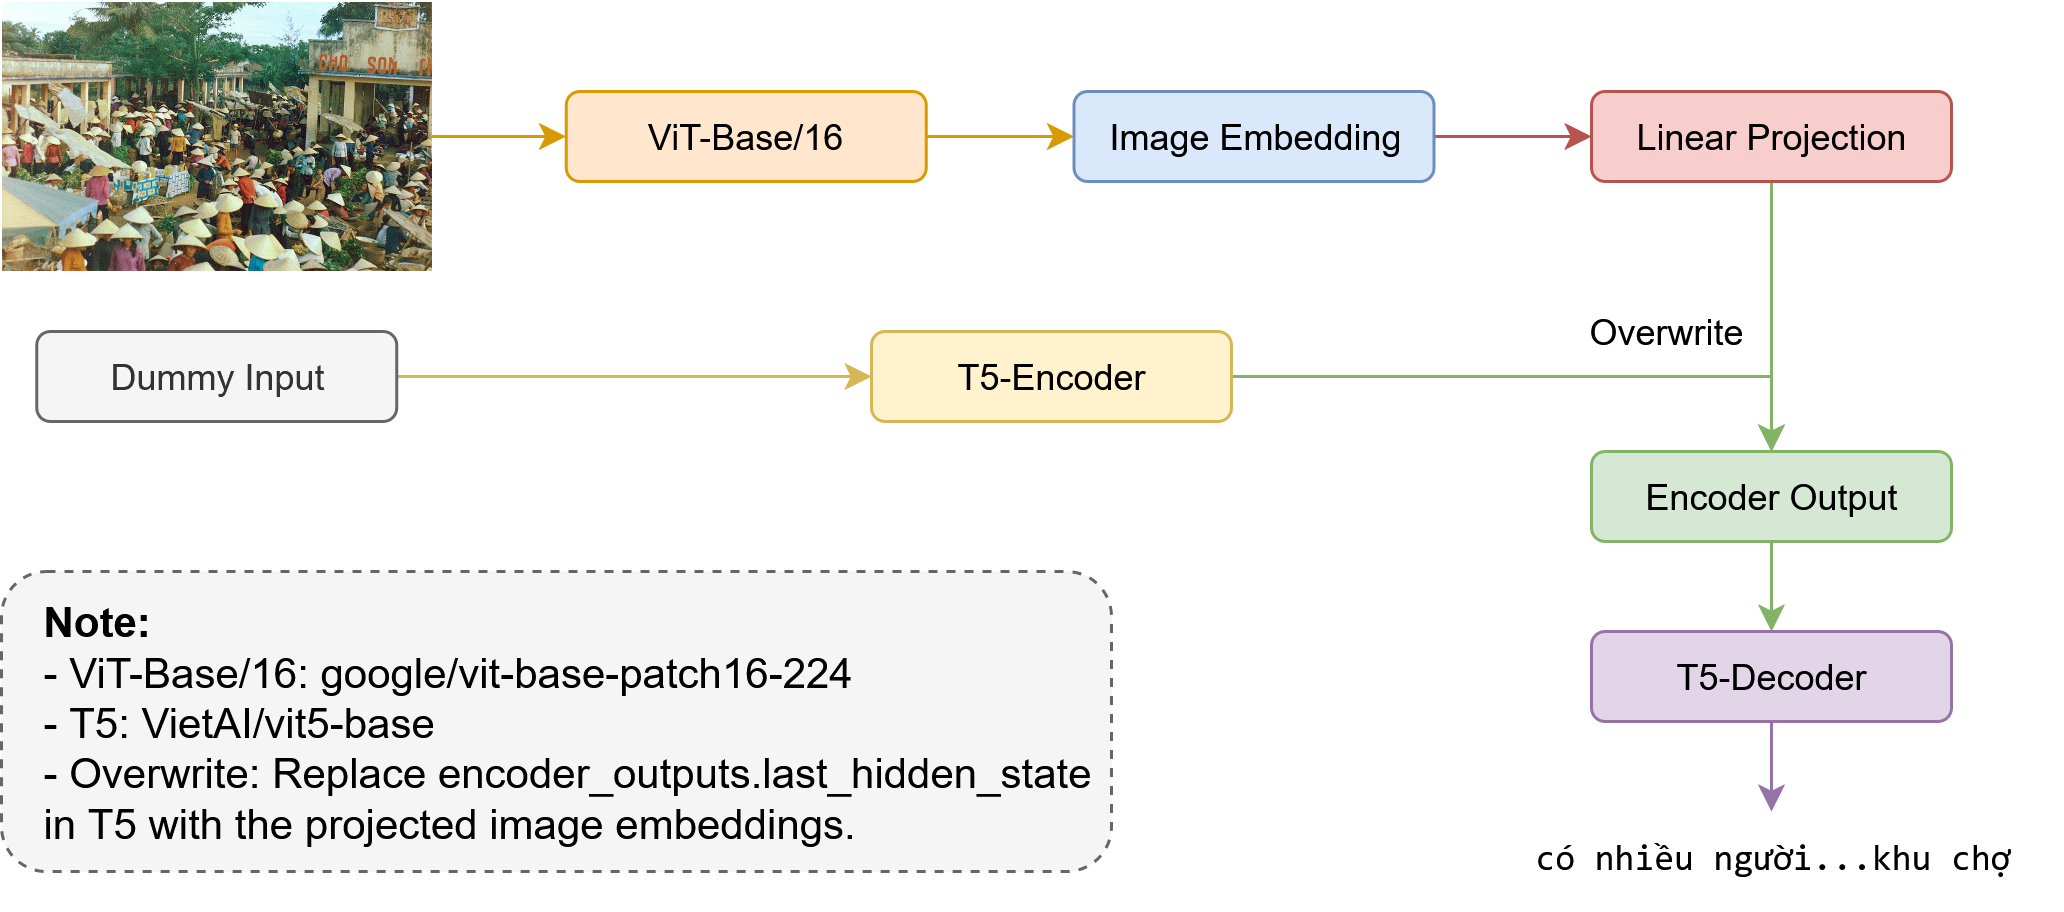
\includegraphics[width=\textwidth]{image/img-captioning-archi.png}
  \caption{The architecture of the ViT-T5 image captioning model, illustrating the integration of the Vision Transformer (ViT) encoder and the T5 decoder.}
  \label{fig:img_cap_archi}
\end{figure}



The visual encoder is a ViT-Base/16~\cite{google-vit-base-patch16-224} model, pre-trained on the ImageNet-21k dataset. Its function is to process an input image and generate a sequence of patch embeddings, which serve as a rich, high-dimensional representation of the image's content.

The text decoder is based on the VietAI/vit5-base~\cite{phan-etal-2022-vit5} model, a T5 variant specifically pre-trained for the Vietnamese language. To bridge the modality gap between the visual encoder and the text decoder, a dedicated interface mechanism was implemented. A linear projection layer maps the embedding dimension of the ViT's output features to the expected hidden dimension ($d_{\text{model}}$) of the T5 decoder.

During the forward pass, the projected visual features directly substitute the output of the T5's own text encoder. Consequently, the T5 decoder's cross-attention mechanism attends directly to this sequence of visual embeddings, enabling it to generate a textual description conditioned on the image content. For generation, the model utilizes a beam search with a beam width of 3 to produce fluent and coherent captions.

\subsubsection{Training Procedure}
The model was trained using a parameter-efficient fine-tuning (PEFT) strategy to leverage the knowledge from the pre-trained components while minimizing computational cost and the risk of catastrophic forgetting. During this phase, the weights of the entire ViT encoder and the T5 text encoder were frozen and did not receive updates. Only the parameters of the T5 decoder, the final language model head, and the intermediary linear projection layer were made trainable.

The model was optimized by minimizing the standard cross-entropy loss between the predicted token sequence and the ground-truth captions. We employed the AdamW optimizer with an initial learning rate of $5 \times 10^{-5}$ and a weight decay of $1 \times 10^{-4}$. The learning rate was dynamically adjusted throughout training using a Cosine Annealing schedule with warm restarts.

Training was conducted for a maximum of 8 epochs. To prevent overfitting and select the best-performing model, an early stopping criterion was implemented. This mechanism monitored the validation loss at the end of each epoch and terminated the training process if no improvement was observed for 5 consecutive epochs. The model checkpoint that achieved the lowest validation loss was saved and used for all subsequent evaluations and inference tasks.



\section{Experiments}

\subsection{Experimental Settings}

\subsubsection{Datasets}

The \textbf{MSVD} dataset (Microsoft Research Video Description) was used as the evaluation benchmark. MSVD contains 1,970 short YouTube video clips (10-25 seconds each) with roughly 80,000 English sentences (about 40 captions per clip). These videos are split following standard practice: 1,200 clips for training, 100 for validation, and 670 for testing. (All captions are in English and describe a single-activity scene per clip, as in prior work.)

\subsubsection{Feature extraction}

For MSVD, we extract both spatial and motion features from the video clips. Video frames were sampled at \textbf{5 frames per second (fps)} and fed into a pretrained \textit{Inception-ResNet-V2} network to obtain \textbf{image features}. Concurrently, videos were resampled at \textbf{25 fps} and divided into overlapping 64-frame segments (stride of 5 frames); these segments were processed by an \textit{Inflated 3D ConvNet (I3D)} to compute \textbf{motion features}. The resulting image and motion feature vectors have dimensions \textbf{2048} and \textbf{1024}, respectively. We also encode each video's category label using a 300-dimensional GloVe word vector. For MSVD, 50 frames are uniformly sampled from each video's features, and all feature vectors (image, motion, and category) are projected to a 512-dimensional space.

\subsubsection{Evaluation metrics}

Performance on MSVD was measured with standard automatic captioning metrics: \textbf{BLEU}, \textbf{METEOR}, \textbf{CIDEr-D}, and \textbf{ROUGE-L}. BLEU and METEOR (originally developed for machine translation) quantify the quality of generated text by n-gram overlap with reference captions. CIDEr-D, explicitly designed for caption evaluation, measures consensus with human annotations. ROUGE-L (longest-common-subsequence based) was also used; it emphasizes recall in overlap between generated and reference sentences. These metrics together provide a comprehensive assessment of caption accuracy, relevance, and fluency.

\subsubsection{Parameter settings}

We detail the model's settings for MSVD experiments. The object detector (Mask R-CNN) used a confidence threshold of 0.7 and minimum box size of 224x224. A TransE knowledge-graph was built from 613 unique triples, with each relationship encoded by a 300-dimensional GloVe vector. The Transformer encoders and decoders use 4 layers, with 640-dimensional input embeddings, 512-dimensional model hidden states, 2048-dimensional feedforward layers, and 10 attention heads per layer. (An extended multi-head attention in the STE component uses 128 heads.) During training on MSVD, the balance weight $\lambda$ between forward/backward decoding was set to 0.6 and the model was trained for 30 epochs. We used the Adam optimizer with a batch size of 32 and a learning rate of 1e-4 for MSVD training. Inference used beam search of size 5 with dropout 0.1. All experiments were run on NVIDIA Tesla P100 GPUs.

\subsection{Performance comparison}

We evaluated our proposed enhancements on the MSVD dataset. The table below presents a comparison between the results published in the original paper, our re-implemented baseline, and our enhanced models.

\begin{table}[H]
  \centering
  \caption{Performance comparison of BTKG models on MSVD dataset.}
  \label{tab:model_comparison}
  \begin{tabular}{|l|c|c|c|c|}
    \hline
    \textbf{Model Version} & \textbf{BLEU@4} &
    \textbf{METEOR} & \textbf{ROUGE-L} & \textbf{CIDEr-D} \\
    \hline
    \textbf{Published Results} & 55.7 & 38.3 & 74.7 & 104.5   \\
    BTKG (Our Baseline) & 54.6 & 37.9 & 74.3 & 96.8    \\
    BTKG + Feature Fusion & 55.1 & 38.0 & 74.1 & 98.1    \\
    BTKG + Feature Fusion + ResiDual & 55.5   & 38.3   & 74.9    & 100.2   \\
    \hline
  \end{tabular}
\end{table}

\subsubsection{Analysis of Results}

\paragraph{Comparison with Published Baseline:} Our re-implementation of the original BTKG model yielded slightly lower scores than those reported in the paper, most notably a drop in the CIDEr-D score from 104.5 to 96.8. This discrepancy can be attributed to differences in the experimental environment (the original paper used an RTX 3060 GPU, whereas our experiments were run on an NVIDIA Tesla P100 on Kaggle) or minor variations in data preprocessing. Nonetheless, this result serves as a solid baseline for evaluating our proposed improvements.

\paragraph{Effectiveness of the Feature Fusion Module:} Replacing element-wise addition with our learnable \textbf{Feature Fusion} module led to a noticeable improvement across most metrics, especially CIDEr-D, which increased from 96.8 to 98.1. This confirms that a learnable, weighted combination of features is more effective than a simple, static summation. The model can better prioritize more relevant information, resulting in a richer fused feature vector for the decoder.

\paragraph{Positive Impact of the ResiDual Architecture:} The most significant improvement came from integrating the \textbf{ResiDual} architecture. The ``\textbf{BTKG + Feature Fusion + ResiDual}'' model substantially outperformed our baseline across all metrics. Notably, the CIDEr-D score saw a strong increase to 100.2, and the METEOR score reached 38.3, matching the published result. By stabilizing the training process and preventing representation collapse, ResiDual allows the deeper layers of the model to learn more complex and diverse representations. This directly enhances the model's ability to capture the fine-grained semantics of the video, leading to more accurate and semantically appropriate captions, as reflected by the significant gain in the CIDEr-D score.

\subsubsection{Conclusion}

While our best-performing model has not yet surpassed all the scores from the original publication, our experimental results clearly demonstrate that:

\begin{enumerate}
    \item Using a learnable mechanism like \textbf{Feature Fusion} is more effective for combining multimodal features than direct summation.
    
    \item Upgrading the Transformer architecture to a more stable and powerful design like \textbf{ResiDual} yields significant performance gains, particularly in the semantic quality of the generated captions.
\end{enumerate}

These findings validate our research direction and show that the proposed enhancements have great potential for improving the overall effectiveness of the BTKG model for video captioning.

\section{Applications}

We investigated the applications of our model across various domains. The model's ability to generate coherent and contextually relevant text makes it suitable for question-answering tasks with a chatbot.



\subsection{Chatbot Application}

We used Gemini 2.5 Flash~\cite{comanici2025gemini} to create a chatbot that can answer questions based on the provided context. The chatbot is designed to understand and respond to user queries in a conversational manner, leveraging the model's capabilities to generate human-like responses.

When a user enters a question accompanied by a short video, the video goes through our two-step captioning process--video captioning and keyframe captioning--and the chatbot then answers the question based on the generated captions. The chatbot is capable of understanding the context of the video and providing relevant answers to user queries.

\subsection{User Interface}

% We designed a user-friendly interface for the chatbot, allowing users to interact with it easily. The interface includes a video player for watching the video, a text input box for entering questions, and a chat window for displaying the chatbot's responses. This setup ensures a seamless user experience, enabling users to engage with the chatbot while watching the video.
\section{Reference}
\defbibheading{bibliography}[\refname]{}
\renewcommand*{\bibfont}{\large}
\nocite{*}  
\printbibliography
\end{document}